\section{Images and Figures}

Images can be included in LaTeX documents fairly easily.  However, you must include a package first in your header:

\begin{quote}
	\begin{verbatim}
		\usepackage{graphicx}
	\end{verbatim}
\end{quote}

Then, in your text where you want the graphic, put:
\begin{quote}
	\begin{verbatim}
		\includegraphics[width=5in]{graphics/number_of_firms.eps}
	\end{verbatim}
\end{quote}

The type of graphics you can include depends on your typesetter, but there are two big ones: PDF and EPS.  In most cases, if what you want to include is a graph or diagram, you should be using EPS.  

Sometimes your graphic will be a figure that you want to reference.  In that case, you can wrap the graphic in a figure:

\begin{quote}
	\begin{verbatim}
		\begin{figure}[hbt]
  			\centering
  			\includegraphics[width=5in]{graphics/number_of_firms.eps}
  			\caption{As the number of firms increase...}
  			\label{fig:firms}
  		\end{figure}
	\end{verbatim}
\end{quote}

Which produces this:

\begin{figure}[hbt]
	\centering
  	\includegraphics[width=5in]{graphics/number_of_firms.eps}
  	\caption{As the number of firms increase...}
  	\label{fig:firms}
\end{figure}

The figure options ``[hbt]" tell LaTeX what part of the page the figure can appear (in this case: ``here" - h, ``bottom" - b or ``top" - t).  I can also reference this figure by using \emph{\textbackslash ref\{fig:firms\}}.